\section{Image Quality}
\label{sec:image_quality}

The AOS team has delivered very impressive image quality, showing images with 0.68 arcsec FWHM. If we assume that sources of image degradation add in quadrature and we trust our estimates of atmospheric seeing, this is consistent with reaching the image quality error budget allocation of our full system of 0.400 arcsec.

We are in the process of quantifying the different sources of image degradation. The main ones we're focused on measuring are degradation due to the camera/instrument, static optics, dynamic optics, mount motion, and observatory seeing.

\subsection{Atmospheric Seeing}

We do not currently have a working Rubin DIMM, although there is work being done to repair it. In the meantime, we have a livestream of data from the SOAR RINGS instrument, which is a  next-generation DIMM developed by Andrei Tokovinin and Edison Bustos. We are working on getting direct access to current and historical data for RINGS as well as the Gemini DIMM.

\subsection{Static Optics}

See Section~\ref{sec:aos_commissioning} for more details on the performance of the static optics system.

\subsection{Instrument}

We are taking the measured LSSTCam instrument image degradation to be the same as for ComCam, so 

\subsection{Dynamic Optics}

Dynamic optics contributions are caused by oscillations or motion of the mirrors, causing focus to shift during an exposure. We have accelerometers in the mirror cell and on the top end but have not yet analyzed the data.

\subsection{Observatory Seeing}

The two main contributors to observatory seeing are dome seeing and mirror seeing. We do not have a direct dome seeing monitor but we do have a sonic anemometer.

\subsection{Mount Motion}

There are two main components to image degradation due to mount motion. The first component comes from drift due to tracking errors. As we have not yet completed a full pointing model at all azimuth and elevations, we have not quantified this component yet. The second component of mount motion image degradation is due to tracking jitter. We quantify this by computing the rms deviation of the mount position as measured by the encoders from the position sent by MTPtg. Craig Lage computed the tracking jitter for all ComCam exposures through the 20th of November. From a total of 5311 images, the median image quality impact is 0.004 arcseconds, and 0.38\% of images have an impact to image quality of above 0.05 arcseconds (see Figs.~\ref{fig:jitter}, ~\ref{fig:jitter_1}, ~\ref{fig:jitter_2}). This is well below the budgeted mount jitter error of 0.069 arcsec.

\begin{figure}
  \label{fig:jitter}
  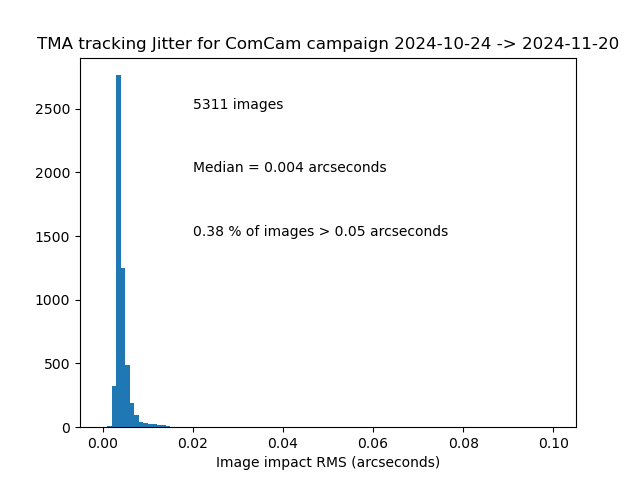
\includegraphics[width=\linewidth]{image_quality_figures/ComCam_Mount_Jitter_21Nov24.png}
  \caption{Total TMA tracking jitter for all exposures from October 24 to November 20.}
\end{figure}

\begin{figure}[h]
    \centering
    \begin{minipage}{0.49\textwidth}
        \centering
        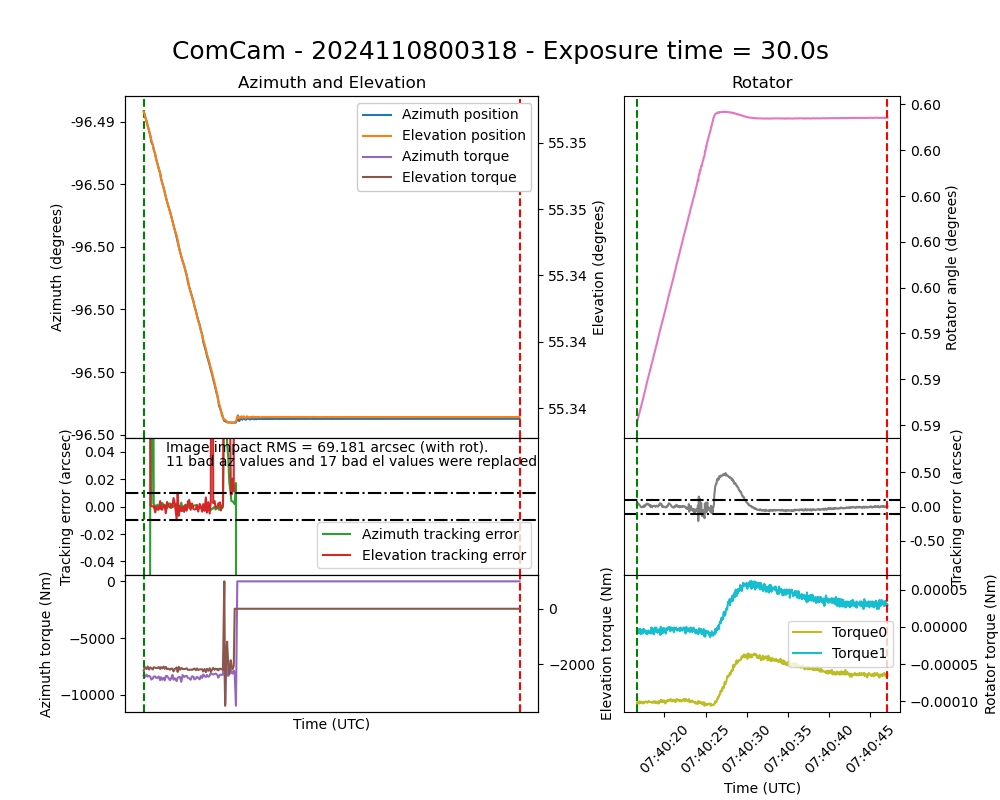
\includegraphics[width=\linewidth]{image_quality_figures/ComCam_Mount_Plot_2024110800318.png}
        \caption{Exposure with an unusually large amount of mount motion image degradation.}
        \label{fig:jitter_1}
    \end{minipage}\hfill
    \begin{minipage}{0.49\textwidth}
        \centering
        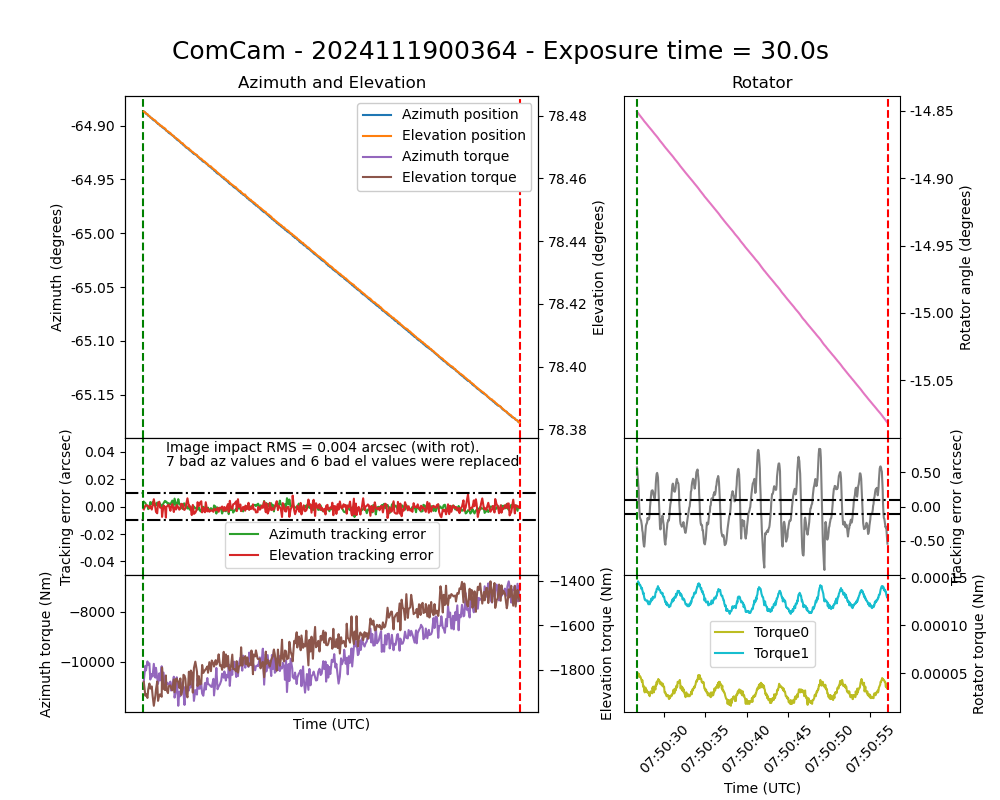
\includegraphics[width=\linewidth]{image_quality_figures/ComCam_Mount_Plot_2024111900364.png}
        \caption{Exposure with a typical amount of mount jitter.}
        \label{fig:jitter_2}
    \end{minipage}
\end{figure}